\documentclass[aspectratio=169,10pt]{beamer}

% Metropolis: modern flat theme
\usetheme{metropolis}
\metroset{progressbar=frametitle, block=fill, numbering=fraction, sectionpage=none}

\usepackage[T1]{fontenc}
\usepackage{lmodern}
\renewcommand{\familydefault}{\sfdefault}

\usepackage{booktabs}
\usepackage{graphicx}
\usepackage{xcolor}
\usepackage{tikz}
\usetikzlibrary{arrows.meta,positioning,fit}

\definecolor{acc}{HTML}{2563EB}
\definecolor{trn}{HTML}{E08A1E}
\definecolor{ink}{HTML}{1B2A3A}

\setbeamercolor{frametitle}{bg=ink}
\setbeamercolor{progress bar}{fg=acc}
\setbeamercolor{alerted text}{fg=trn}
\setbeamercolor{normal text}{fg=ink}

\newcommand{\up}[1]{\textcolor{acc}{\textbf{#1}}}

\title{Making OpenAD Robust to Query Phrasing}
\subtitle{in 3D Affordance Detection}
\author{\scriptsize
  \begin{tabular}{ccc}
    Mehreen Hossain Chowdhury & Sumaiya Ahmed Rani & Jannatul Fardus Rakhi \\
    210041219 & 210041223 & 210041237
  \end{tabular}}
\institute{Dept.\ of CSE, Islamic University of Technology}
\date{}

\begin{document}

\maketitle

% 1. PROBLEM
\begin{frame}{Problem \& contribution}
  \textbf{Affordance detection:} \emph{where} on a 3D object can I act
  (grasp a handle, sit on a seat, cut with a blade)?

  \medskip
  \textbf{OpenAD} handles this as an open-vocabulary task. It matches each point's
  PointNet++ feature to a query embedding from \emph{frozen CLIP}. However, it is trained
  using only \emph{single-word} queries.

  \medskip
  \alert{Users may not say ``grasp.'' They may ask, ``Where can I grasp this object?''}
  How well does the model handle this change in wording?

  \medskip
  \textbf{Our approach} uses pretrained weights and introduces no new architecture:
  \begin{itemize}
    \item reproduce OpenAD and measure its sensitivity to phrasing;
    \item improve its robustness with lightweight prompt-augmented fine-tuning;
    \item provide an interactive demonstration.
  \end{itemize}

  \begin{block}{Headline}
    Rephrasing costs \up{$\sim$12 mIoU}. Fine-tuning \up{101k params (5.7\%)} recovers
    \up{$>$90\%} of that loss on \emph{unseen} wordings while preserving performance on
    canonical words.
  \end{block}
\end{frame}

% 2. DATASET AND EVALUATION
\begin{frame}{Dataset \& evaluation}
  \textbf{3D AffordanceNet} (full-shape, as shipped with OpenAD)
  \begin{itemize}
    \item Each object has 2,048 points and one of \up{19 classes}: 18 affordances plus \texttt{none}.
    \item The validation split contains \up{2{,}285 objects} and is highly imbalanced. Table and Chair make up 62\% of it.
  \end{itemize}

  \textbf{Metrics.} We report per-point \up{mIoU} over 19 classes, point accuracy, and mean
  class accuracy. Our implementation matches OpenAD's evaluator and is covered by unit tests.

  \textbf{Phrasing conditions.} We study five affordances: grasp, contain, sittable, pourable,
  and cut. Each appears as a label, question, or description. The fine-tuning and held-out
  phrase sets were \up{fixed before training}, and a test checks that they do not overlap.

  \textbf{Evaluation noise.} Because farthest-point sampling starts randomly, repeated runs
  vary by about \up{0.4 mIoU}. We treat differences below 0.5 as equivalent.
\end{frame}

% 3. METHOD
\begin{frame}{Method: architecture $+$ our modification}
  \centering
  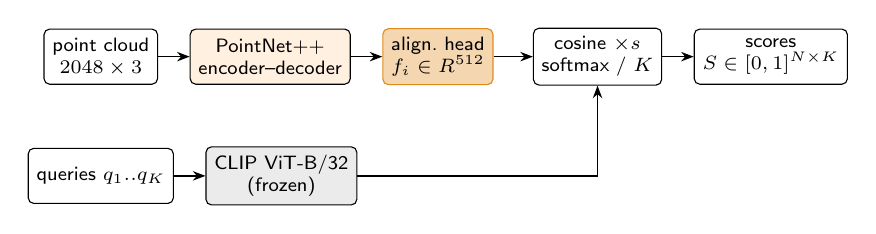
\begin{tikzpicture}[font=\scriptsize,
    box/.style={draw,rounded corners=2pt,minimum height=7mm,align=center,inner sep=3pt},
    frozen/.style={box,fill=black!8},
    bb/.style={box,fill=orange!12},
    train/.style={box,fill=trn!35,draw=trn},
    arr/.style={-{Stealth[length=1.6mm]},line width=0.5pt}]
    \node[box] (pc){point cloud\\$2048\times3$};
    \node[bb,right=4mm of pc] (enc){PointNet++\\encoder--decoder};
    \node[train,right=4mm of enc] (head){align.\ head\\$f_i\in\mathbb{R}^{512}$};
    \node[box,right=5mm of head] (al){cosine $\times s$\\softmax / $K$};
    \node[box,right=4mm of al] (sc){scores\\$S\in[0,1]^{N\times K}$};
    \node[box,below=8mm of pc,align=center] (q){queries $q_1..q_K$};
    \node[frozen,right=4mm of q] (clip){CLIP ViT-B/32\\(frozen)};
    \foreach \a/\b in {pc/enc,enc/head,head/al,al/sc}{\draw[arr] (\a)--(\b);}
    \draw[arr] (q)--(clip);
    \draw[arr] (clip.east) -| (al.south);
  \end{tikzpicture}

  \smallskip
  {\scriptsize \textcolor{trn}{$\blacksquare$}~trainable (head $+$ last prop.\ layer, 101k)\quad
   \textcolor{orange!60!black}{$\blacksquare$}~frozen backbone\quad
   \textcolor{black!45}{$\blacksquare$}~frozen CLIP}

  \medskip
  \begin{columns}[T]
    \column{0.48\textwidth}
    \textbf{Unchanged from OpenAD}
    \begin{itemize}\footnotesize
      \item cosine align $\times$ learnable scale $s$, softmax
      \item class-weighted NLL (cube-root inv-freq)
      \item Adam
    \end{itemize}
    \column{0.52\textwidth}
    \textbf{Our modification: prompt-augmented fine-tuning}
    \begin{itemize}\footnotesize
      \item At each step, sample one paraphrase for every studied affordance. Labels and loss remain unchanged.
      \item Train only the \up{head and fp1} (5.7\% of the network) for 8 epochs at LR $10^{-4}$.
      \item Select the epoch using canonical validation mIoU, without using held-out phrases.
    \end{itemize}
  \end{columns}
\end{frame}

% 4. SETUP AND BASELINES
\begin{frame}{Experimental setup \& baselines}
  \begin{columns}[T]
    \column{0.5\textwidth}
    \textbf{Models compared}
    \begin{itemize}\small
      \item majority-class and random baselines
      \item pretrained OpenAD from a pinned commit
      \item our fine-tuned models at three capacities
    \end{itemize}
    \textbf{Capacity ladder} (same data/seed):\\
    head 67k $\to$ head$+$fp1 101k $\to$ decoder 743k.
    \column{0.5\textwidth}
    \textbf{Fair comparison}
    \begin{itemize}\small
      \item Both models are evaluated in the same script run.
      \item They use the same objects, order, metrics, and query lists.
      \item \up{Only the model weights differ} in the model comparison.
    \end{itemize}
    \textbf{Implementation}
    \begin{itemize}\small
      \item PyTorch 2.5 / CUDA 12.1, 1$\times$ RTX 4060
      \item $\sim$14 min/epoch; 16 unit tests
    \end{itemize}
  \end{columns}
\end{frame}

% 5. REPRODUCTION
\begin{frame}{Reproduction validates the harness}
  \centering\small
  \begin{tabular}{@{}llccc@{}}
    \toprule
    Setting & Method & mIoU & Acc & mAcc \\
    \midrule
    Closed-set & OpenAD (cited) & 42.00 & 69.03 & 67.31 \\
               & \up{ours} & 41.25 & 68.51 & 66.73 \\
    \midrule
    Open-vocab & ZSLPC (cited) & 9.97 & 40.13 & 18.70 \\
               & OpenAD (cited) & 14.37 & 46.31 & 19.51 \\
               & \up{ours} & \up{14.40} & 46.33 & 19.63 \\
    \midrule
    Floor & majority (\texttt{none}) & 2.27 & 43.04 & 5.26 \\
          & random & 1.47 & 5.28 & 5.43 \\
    \bottomrule
  \end{tabular}

  \medskip
  {\footnotesize Our open-vocabulary score of \up{14.40} closely matches the reported 14.37.
  The majority baseline reaches 43\% point accuracy but only 2.27 mIoU, showing why mIoU is
  more informative for this imbalanced dataset.}
\end{frame}

% 6. SENSITIVITY
\begin{frame}{The problem: phrasing breaks the pretrained model}
  \begin{columns}[c]
    \column{0.42\textwidth}
    \small
    \begin{tabular}{@{}lccc@{}}
      \toprule
      Affordance & Canon. & Ques. & Descr. \\
      \midrule
      grasp    & 42.6 & 0.0  & 0.4 \\
      contain  & 43.9 & 0.0  & 0.3 \\
      sittable & 59.6 & 2.0  & 21.8 \\
      pourable & 41.5 & 0.0  & 0.0 \\
      cut      & 55.2 & 43.2 & 37.1 \\
      \midrule
      \up{mIoU (19)} & \up{41.5} & \up{29.6} & \up{30.3} \\
      \bottomrule
    \end{tabular}
    \column{0.58\textwidth}
    \footnotesize
    Rephrasing the queries as questions or descriptions reduces mIoU by about \up{12 points}.\\[5pt]
    Grasp, contain, and pourable fall close to zero, while \emph{cut} remains relatively strong.\\[5pt]
    The score maps are still \emph{spatially correlated} (Pearson 0.60--0.89), which suggests
    that the main weakness lies in \up{alignment} rather than spatial feature extraction.
  \end{columns}
\end{frame}

% 7. RESULTS
\begin{frame}{Results: fine-tuning recovers the loss}
  \begin{columns}[T]
    \column{0.44\textwidth}
    \small
    \begin{tabular}{@{}lccc@{}}
      \toprule
      Condition & Pre & FT & $\Delta$ \\
      \midrule
      Canonical                     & 41.3 & 42.0 & $+0.7$ \\
      Question, seen                & 29.0 & 42.1 & $+13.1$ \\
      \textbf{Question, held-out}   & 29.3 & \up{40.5} & \up{$+11.2$} \\
      Description, seen             & 29.6 & 42.4 & $+12.7$ \\
      \textbf{Descr., held-out}     & 30.4 & \up{40.9} & \up{$+10.5$} \\
      \bottomrule
    \end{tabular}

    \medskip
    \footnotesize
    \begin{itemize}
      \item Recovers \up{93\%} and \up{96\%} of the loss.
      \item Held-out scores are only about 1.5 points below seen scores, suggesting generalisation rather than memorisation.
      \item Preserves canonical-word performance ($+0.7$).
    \end{itemize}
    \column{0.56\textwidth}
    \centering
    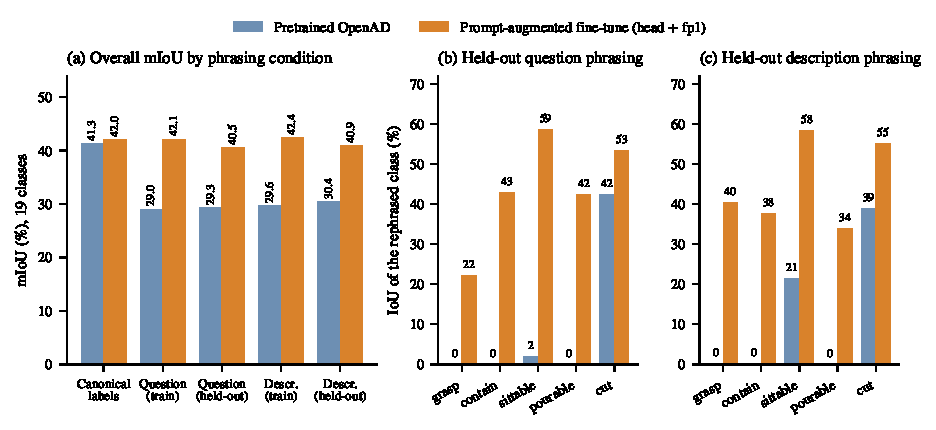
\includegraphics[width=\linewidth]{figures/fig_results.pdf}
  \end{columns}
\end{frame}

% 8. ABLATION
\begin{frame}{Ablation: how much of the network to train?}
  \centering\small
  \begin{tabular}{@{}lcccc@{}}
    \toprule
    Model & Params & Canon. & Q held-out & D held-out \\
    \midrule
    Head only             & 67{,}073  & $+0.49$ & $+10.53$ & $+10.04$ \\
    Head$+$fp1 (reported) & 101{,}377 & $+0.74$ & \up{$+11.21$} & \up{$+10.48$} \\
    Decoder (fp1--fp3)    & 743{,}041 & $+0.54$ & $+10.91$ & $+10.28$ \\
    \bottomrule
  \end{tabular}

  \medskip
  \begin{columns}[T]
    \column{0.5\textwidth}\footnotesize
    $\Delta$ vs.\ each rung's own pretrained run.\\
    Head alone already gives $+10.5/+10.0$.
    \column{0.5\textwidth}\footnotesize
    Performance stays nearly constant across an \up{$11\times$ parameter range}. Most of the
    improvement therefore comes from the alignment head, so the encoder can remain frozen.
  \end{columns}
\end{frame}

% 9. TRAINING AND OPEN-VOCABULARY TRANSFER
\begin{frame}{Training behaviour \& open-vocabulary transfer}
  \begin{columns}[T]
    \column{0.42\textwidth}
    \centering\footnotesize
    \begin{tabular}{@{}ccc@{}}
      \toprule
      Epoch & Loss & Val mIoU \\
      \midrule
      1 & 0.701 & 41.72 \\
      \textbf{4} & 0.644 & \up{42.46} \\
      8 & 0.639 & 42.15 \\
      \bottomrule
    \end{tabular}\\[4pt]
    {\scriptsize Validation mIoU peaks at epoch 4 and remains stable afterwards.}
    \column{0.58\textwidth}
    \centering\footnotesize
    \begin{tabular}{@{}lccc@{}}
      \toprule
      Synonym & Pre & FT & $\Delta$ \\
      \midrule
      grasp (grab)           & 1.7  & 36.3 & $+34.6$ \\
      sittable (take a seat) & 26.2 & 57.9 & $+31.7$ \\
      contain (accommodate)  & 0.2  & 0.0  & $-0.2$ \\
      13 unstudied (mean)    & 9.22 & 9.17 & $-0.05$ \\
      \midrule
      \up{mIoU (19)}         & 14.40 & \up{18.66} & $+4.26$ \\
      \bottomrule
    \end{tabular}\\[4pt]
    {\scriptsize The five fine-tuned affordances account for 97\% of the gain. The other classes remain stable.}
  \end{columns}
\end{frame}

% 10. PER-CLASS RESULTS
\begin{frame}{Per-class IoU: canonical vs.\ synonym}
  \centering
  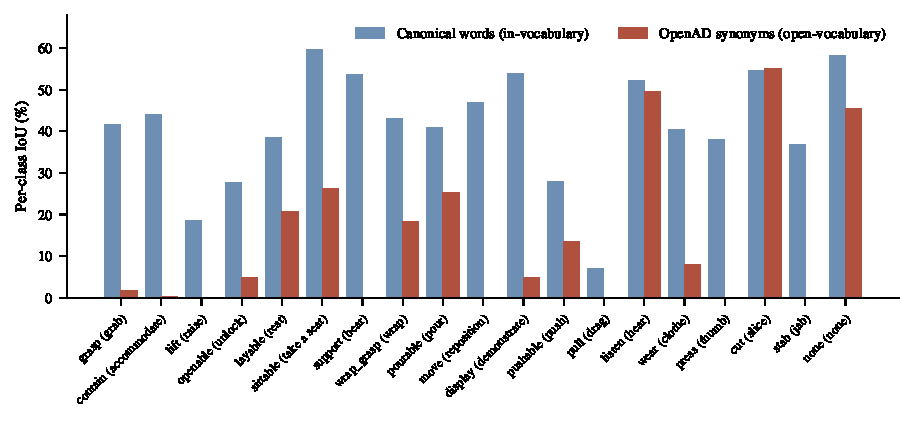
\includegraphics[width=0.9\textwidth]{figures/fig_perclass.pdf}\\
  {\footnotesize Ten of 18 synonyms fall below 5\% IoU; two (slice, hear) nearly match the
  canonical word. Transfer is therefore \up{non-uniform} and depends on the chosen synonym.}
\end{frame}

% 11. QUALITATIVE RESULTS AND DEMO
\begin{frame}{Qualitative, failure cases \& demo}
  \begin{columns}[T]
    \column{0.6\textwidth}
    \centering
    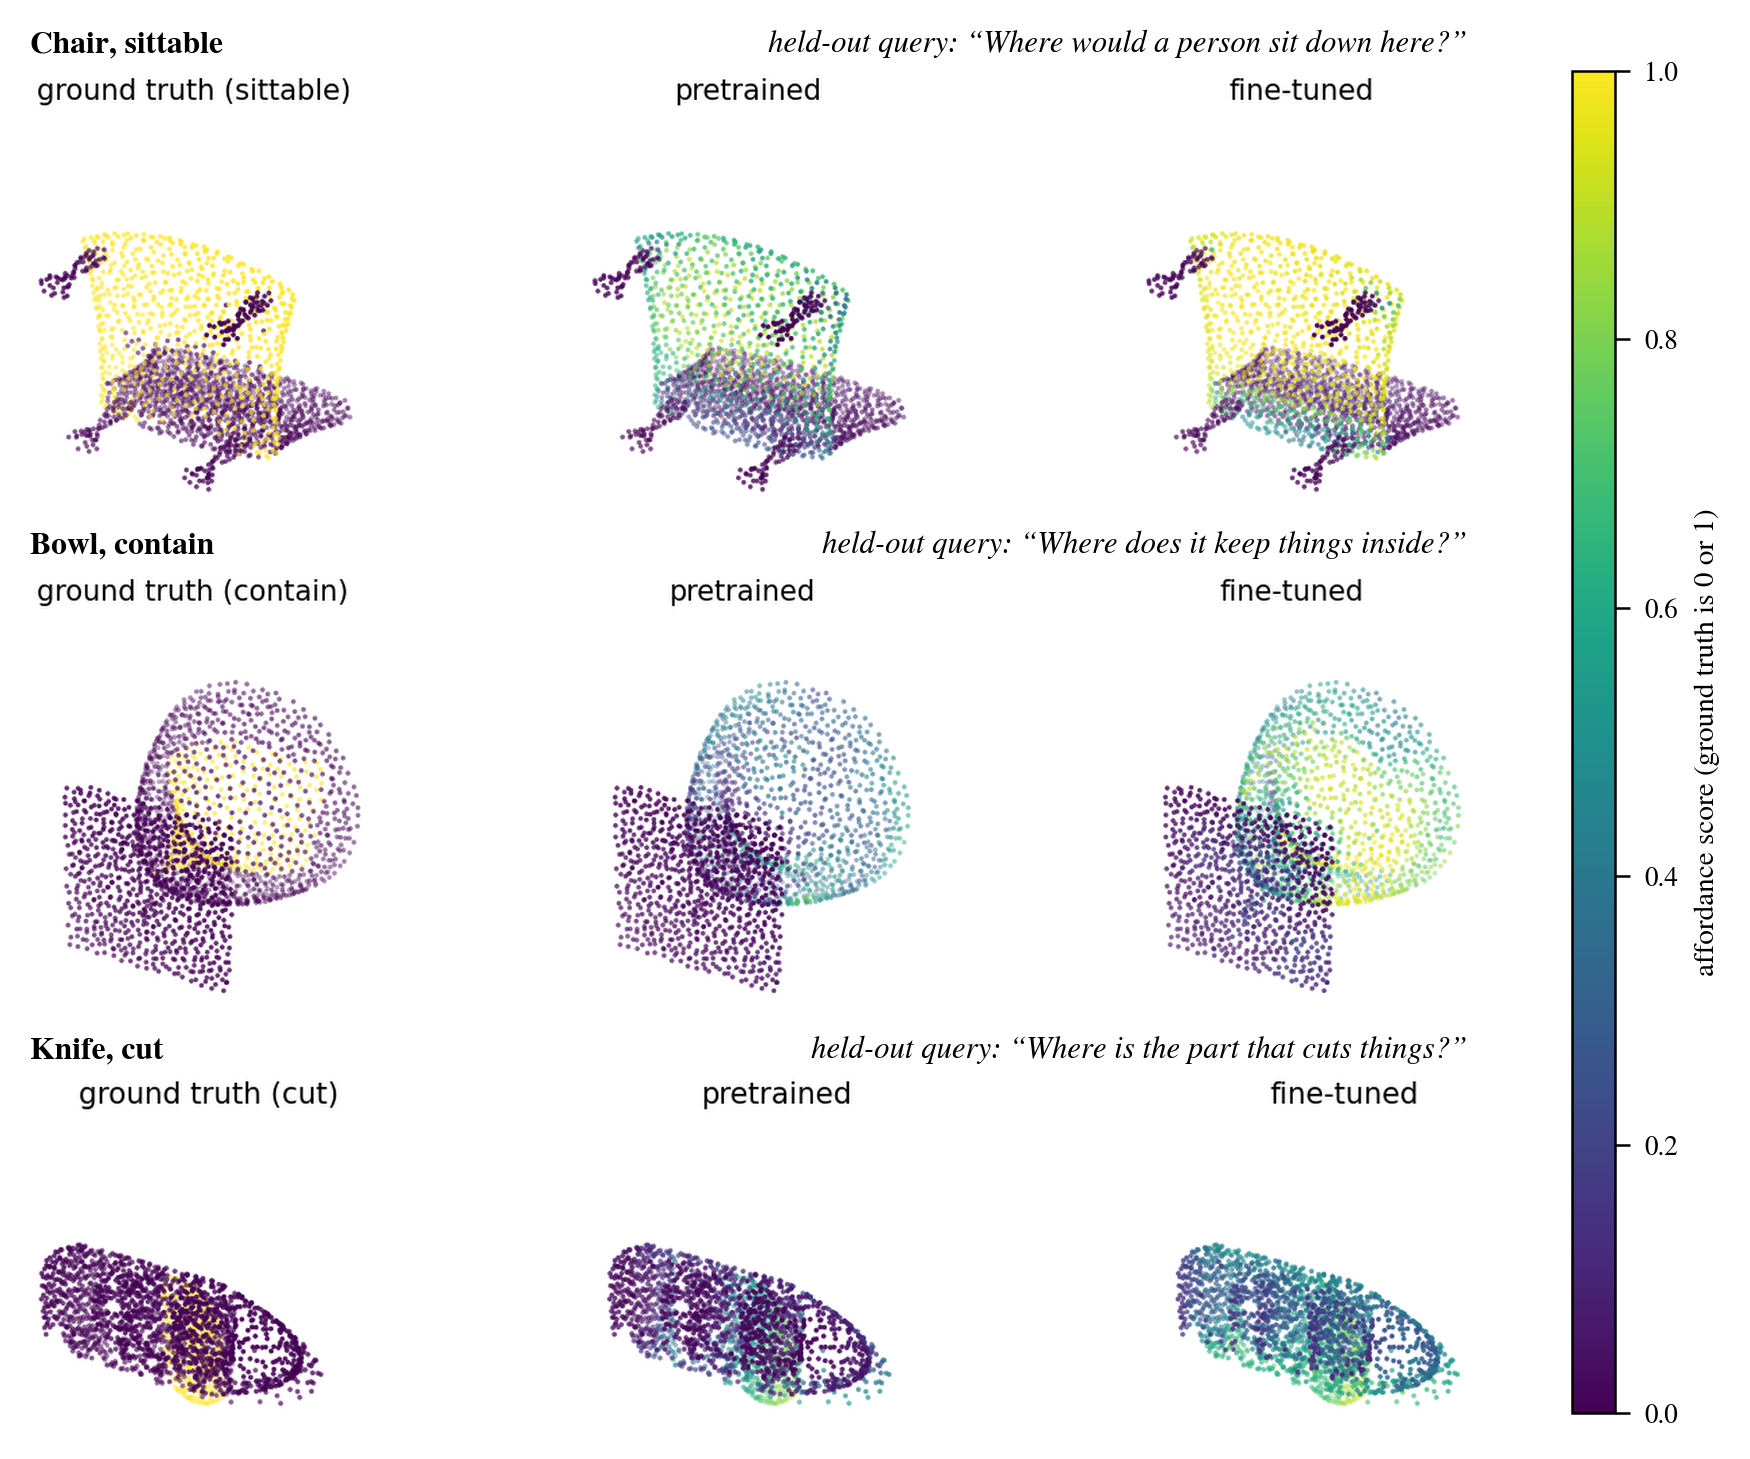
\includegraphics[width=\linewidth]{figures/fig_qual_a.png}\\
    {\scriptsize ground truth $\;|\;$ pretrained $\;|\;$ fine-tuned \quad (held-out question)}
    \column{0.4\textwidth}
    \footnotesize
    \textbf{Successes:} The chair and bowl regions are recovered, and the knife has a sharper peak.\\[3pt]
    \textbf{Failure:} Neither model detects the grasp region of the bag. The split contains only
    12 bags, and their handles vary considerably.\\[5pt]
    \textbf{Demo:} The Gradio and Plotly interface lets users choose an object and model, enter a
    query, inspect a rotatable heat map, compare phrasings, and identify low-confidence results.
  \end{columns}
\end{frame}

% 12. CONCLUSION
\begin{frame}{Conclusion}
  \begin{itemize}
    \item We reproduced OpenAD (\up{14.40} vs. 14.37). Natural rephrasing of five affordances reduces performance by about \up{12 mIoU}.
    \item \up{Prompt-augmented fine-tuning} of 101k params (5.7\%) recovers \up{93--96\%} on
      \emph{held-out} wordings, preserves canonical performance, and improves the synonym benchmark from 14.40 to 18.66.
    \item The alignment head provides most of the gain across an $11\times$ parameter range,
      indicating that the main mismatch is in \up{point-to-text alignment} rather than geometry.
  \end{itemize}
  \textbf{Limitations and next steps:} five affordances, ten held-out phrases, and one seed.
  Future work should test more prompts and seeds, evaluate synonyms at every depth, and explore
  objectives that encourage consistent predictions across paraphrases.
\end{frame}

\begin{frame}[standout]
  Thank you. Questions?\\[4pt]
  {\normalsize\normalfont github.com/mehreen019/Open-Vocabulary-3D-Affordance-Detection}
\end{frame}

\end{document}
